% 第 5 周交付物:ML 架构设计文档(中文版) —— 编译方式:XeLaTeX
\documentclass[11pt]{ctexart}
\usepackage[a4paper, margin=2.4cm]{geometry}
\usepackage{amsmath}
\usepackage{booktabs}
\usepackage{graphicx}
\usepackage[hidelinks]{hyperref}
\usepackage{enumitem}
\setlist{nosep}

\title{\textbf{机器学习架构设计文档}\\
\large Advanced Chooser Option Pricing Model --- 第 5 周交付物}
\author{佟铸城 (Zhucheng Tong)}
\date{2026 年 8 月}

\begin{document}
\maketitle

\section{两条技术路线}
\begin{center}
\small
\begin{tabular}{p{2.0cm} p{5.6cm} p{6.4cm}}
\toprule
& \textbf{路线 A:波动率预测 + BSM} & \textbf{路线 B:端到端定价} \\
\midrule
预测目标 & 期权存续期(1 年)内\textbf{实际实现}的波动率 $\sigma_{oracle}$ & oracle 价格 / 现价(无量纲化,避免学到``价格随股价涨''的平凡关系) \\
定价方式 & 预测 $\hat\sigma$ 代入 chooser 闭式解 & 预测值 $\times$ 现价 \\
初版模型 & Ridge / RandomForest / GBDT / LSTM(63 日序列) & Ridge / GBDT / MLP \\
优点 & 保留无套利结构,可解释($\hat\sigma$ 有含义) & 不受 BSM 函数形式束缚 \\
风险 & 上限受 BSM 形式限制 & 无套利无保证,外推不稳定 \\
\bottomrule
\end{tabular}
\end{center}
说明:GBDT 采用 sklearn HistGradientBoosting(与 XGBoost 同族的梯度提升树、直方图实现;XGBoost 依赖 libomp 系统库,本机不可用,W6 若需要可补装对照)。

\section{数据切分:70/15/15 + 净化(purging)}
按时间顺序切分 1310 个交易日的定价面板:训练 917 行、验证 196 行(2023-06 至 2024-03)、测试 198 行(2024-03 至 2024-12)。\textbf{两个防泄漏设计}:
\begin{enumerate}
  \item \textbf{净化}:目标变量向前看 252 个交易日,训练集尾部 252 行被删除(实际训练 664 行,截至 2022-06),保证任何训练标签的未来窗口都不越过验证边界;
  \item \textbf{测试集本周不开封}:所有模型选择只基于验证集,测试集将在第 6 周调参完成后\textbf{只打开一次}。测试集天然干净——其标签用 2025 年的价格,任何模型输入都未见过。已如实记录的一处妥协:验证集标签窗口与测试集特征期重叠(仅影响超参选择,不影响测试完整性)。
\end{enumerate}
特征工程适配:线性模型使用剔除共线对($|\rho|>0.95$:\texttt{r\_3m}、\texttt{parkinson\_vol\_21d})后的 16 特征并标准化(scaler 只在净化后的训练集上拟合);树模型使用全部 18 个原始特征;LSTM 使用 63 日标准化特征序列。

\section{初版实验:一次有教益的失败与一次设计修正}

\subsection{直接预测波动率水平:全军覆没}
七个初版模型在验证集上\textbf{全部大幅输给 EWMA 基线}(综合分 2.0--3.7,MLP 因外推失稳达 90),且失败模式一致:全体正偏差 $+14$ 至 $+26$ 美元。诊断:训练窗(截至 2022-06,被净化截断)被 COVID 与 2022 熊市主导,目标波动率多在 25\%--90\%;验证窗(2023--24)是 15\%--25\% 的低波动状态。\textbf{树模型结构上无法输出低于训练集所见的值},线性与神经网络则被特征分布漂移(如利率从 $\leq2.5\%$ 跃至 $5\%$,训练期从未见过)带偏。

\subsection{设计修正:锚定目标(anchored target)}
将预测目标从波动率\textbf{水平}改为相对 EWMA 锚的\textbf{对数修正量}:
\[
y = \ln\!\big(\sigma_{oracle} / \sigma_{EWMA}\big), \qquad
\hat\sigma = \sigma_{EWMA}\cdot e^{\hat y}.
\]
关键性质:模型输出 0 时\textbf{恰好还原 EWMA 基线}(已写成审计断言逐日验证),即模型只学习``相对当前波动率该往哪个方向修正多少'',状态水平的漂移被锚吸收。这与第 3 周条件蒙特卡洛的哲学同源:\textbf{把已知结构(当前波动率水平)从学习任务中剥离,让 ML 只学残差}。

\subsection{锚定后的结果(验证集)}
\begin{center}
\small
\begin{tabular}{lrrrrrr}
\toprule
& \textbf{MAE(\$)} & \textbf{Bias} & \textbf{P95} & \textbf{$R^2$} & \textbf{Hit10} & \textbf{综合分} \\
\midrule
\textbf{锚定 Ridge} & \textbf{3.90} & $-0.46$ & \textbf{8.45} & $-0.07$ & \textbf{35.2\%} & \textbf{0.567} \\
EWMA 基线(参照) & 6.44 & --- & --- & $-1.87$ & 19.4\% & 1.000 \\
最好的水平目标模型 & 13.75 & $+13.8$ & 20.7 & $-8.5$ & 0.5\% & 2.037 \\
\bottomrule
\end{tabular}
\end{center}

\textbf{锚定 Ridge 成为首个全面击败基线的模型}:定价 MAE 下降 39\%,$R^2$ 从 $-1.87$ 拉至 $-0.07$(接近转正),可用天数占比近乎翻倍;波动率预测本身 MAE 3.8 个波动率点(EWMA 持续性预测为 6.0 个点)。诚实的另一面:\textbf{锚定并未拯救树模型}(综合分反而 3.8--4.2)——利率水平特征在验证期严重越出训练分布,树模型落入错误叶节点;这一失败指明了第 6 周的修正方向。

\begin{figure}[h!]
\centering
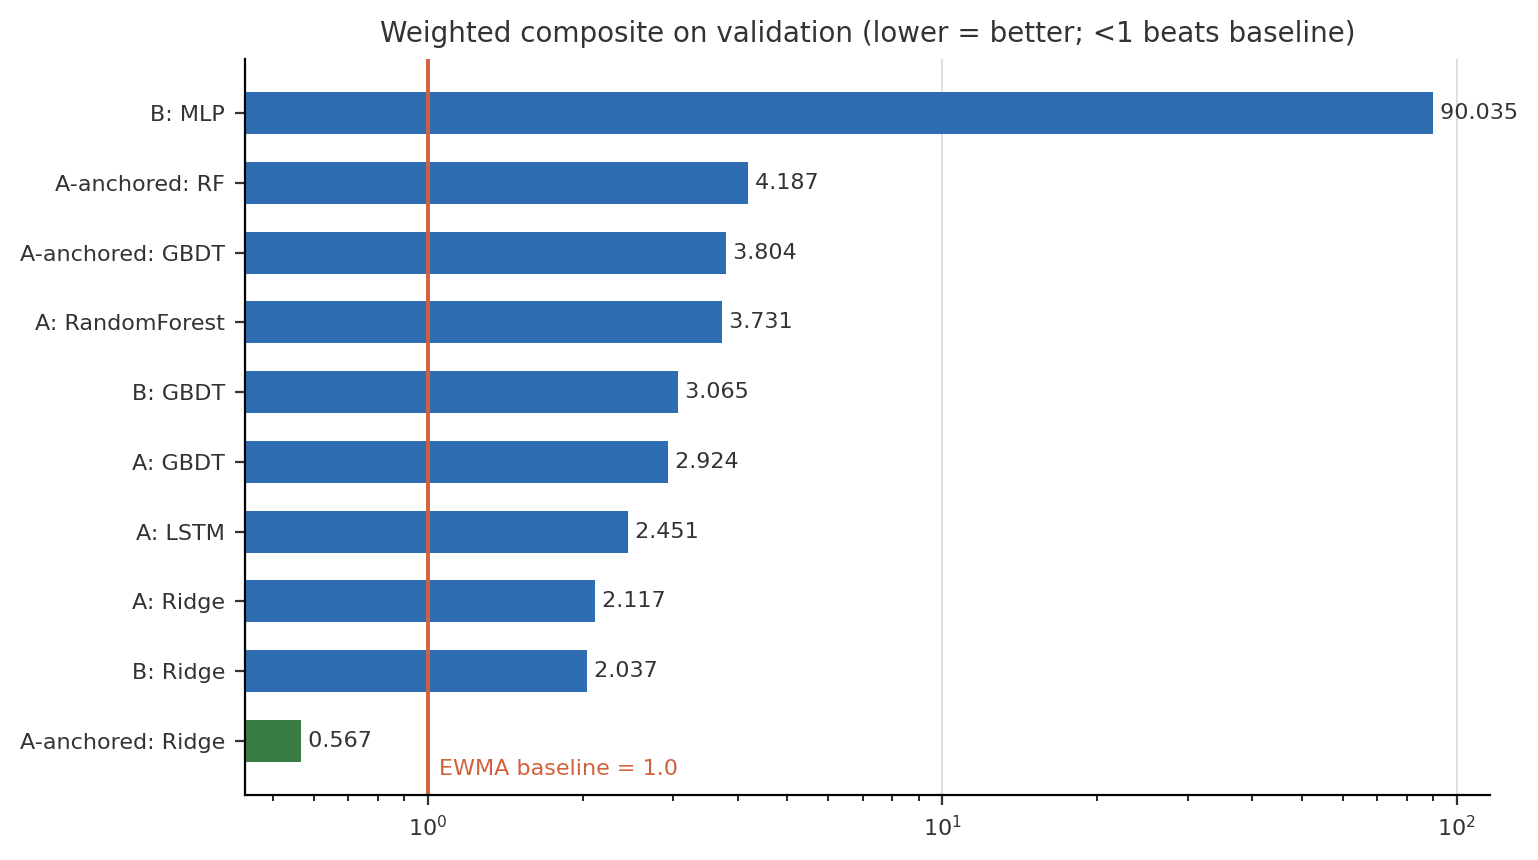
\includegraphics[width=0.8\textwidth]{figures/val_composite.png}
\caption{验证集综合分(对数轴;绿色 $<1$ 为击败基线)}
\end{figure}

\begin{figure}[h!]
\centering
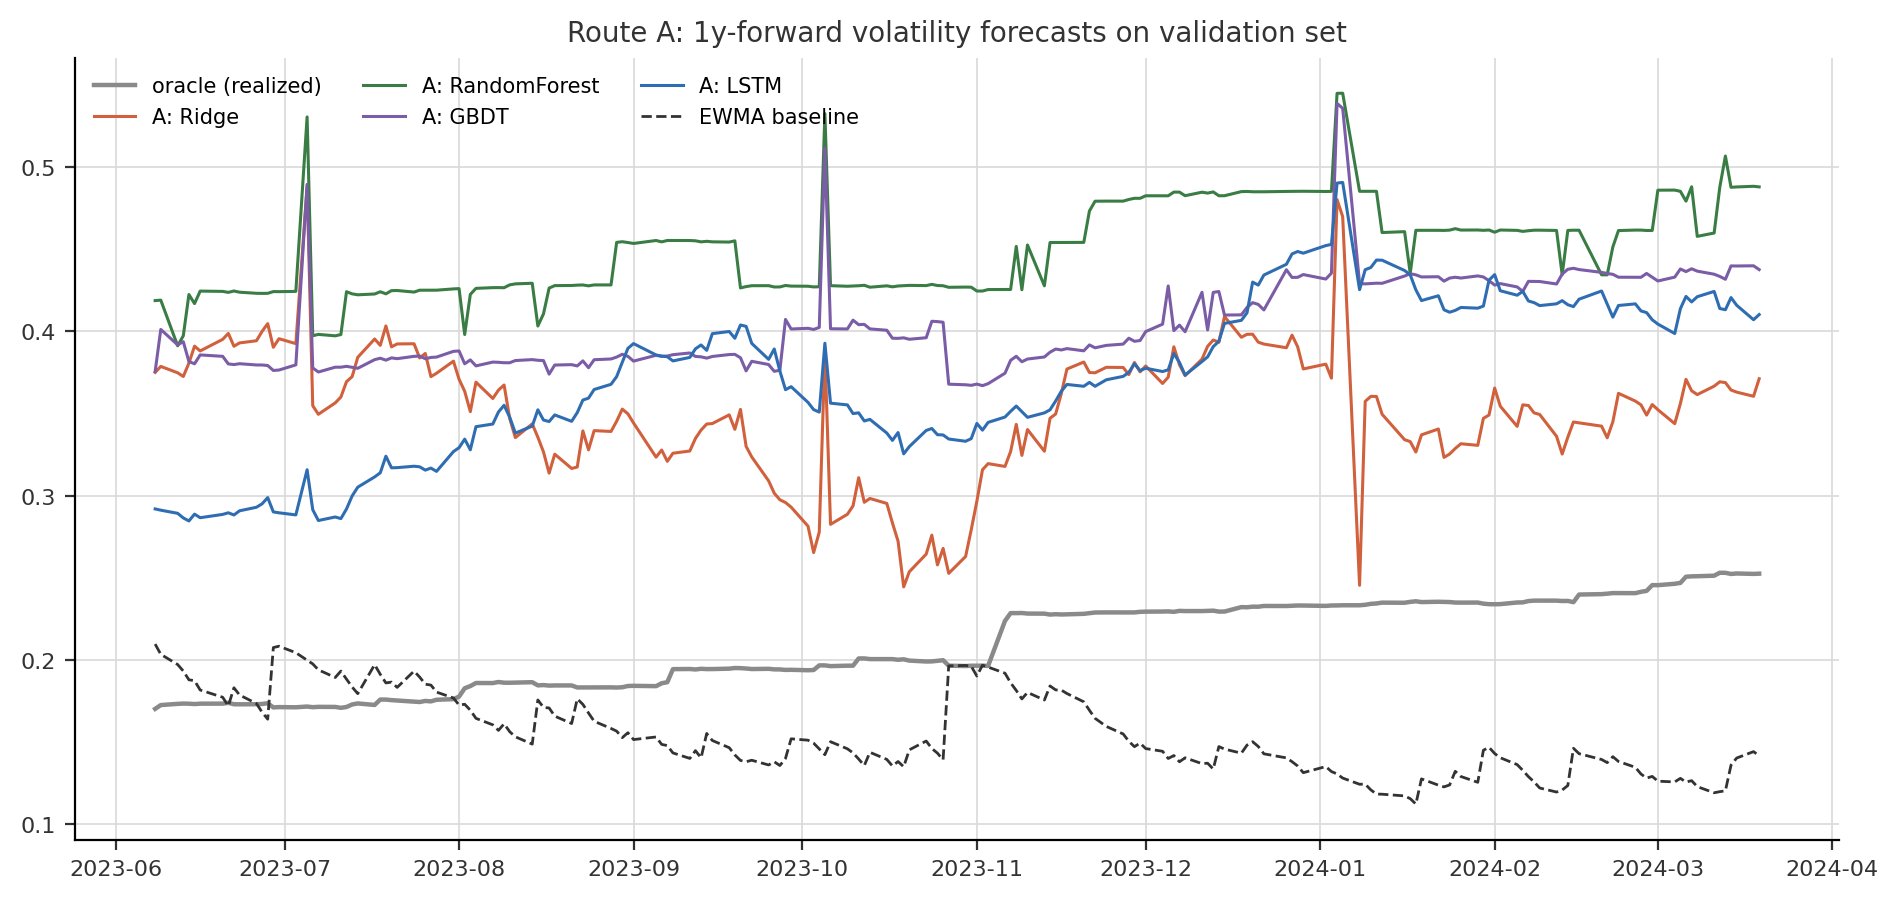
\includegraphics[width=0.94\textwidth]{figures/val_vol_forecasts.png}
\caption{路线 A 各模型在验证集上的波动率预测 vs 事后真值}
\end{figure}

\section{第 6 周计划(训练、调参与对比)}
\begin{enumerate}
  \item \textbf{滚动重训(walk-forward)}:以扩张窗口逐季重训,替代一次性训练——直接解决``训练分布过时''问题,也更贴近实际部署;
  \item \textbf{特征修正}:利率\textbf{水平}特征替换为变化量/相对量(动量、与滚动均值之差),消除树模型的越界外推;
  \item \textbf{超参搜索}:时序交叉验证下的网格/随机搜索(Ridge $\alpha$、树深度/学习率、LSTM 容量),MLP 加鲁棒标准化与目标裁剪;
  \item \textbf{开封测试集}:调参定型后在测试集上\textbf{一次性}评估,报告 8 指标+综合分,并做 SHAP 可解释性分析;
  \item 锚定思想推广到路线 B(预测 $\ln(P_{oracle}/P_{EWMA})$)。
\end{enumerate}

\section{可复现性}
全部训练固定种子(sklearn \texttt{random\_state=42}、torch 手动种子、LSTM 强制 CPU 保证逐位确定);\texttt{python -m src.analysis\_w5} 一键复现;六项防泄漏/一致性审计见 \texttt{analysis/week5/01\_ml\_frameworks.py}(净化间隔、scaler 泄漏、锚定还原恒等式、测试集封存、重训确定性、综合分重算)。初版模型已存 \texttt{models/*.joblib}。

\end{document}
